\documentclass[border=5mm]{standalone}
\usepackage{tikz}

\begin{document}
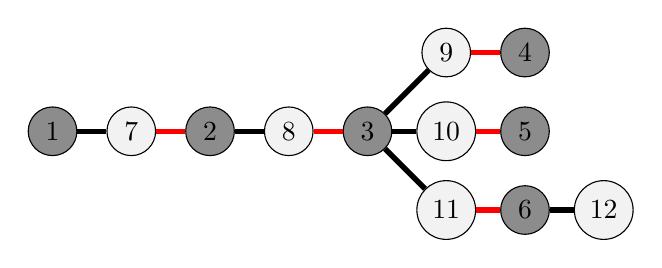
\begin{tikzpicture}[every tree node/.style={draw, circle, inner sep=2pt, text width=1.5em, align=center}]

    \node[draw, fill=gray!90, circle] (1) at (0, 0) {1};
    \node[draw, fill=gray!10, circle] (7) at (1, 0) {7};
    \node[draw, fill=gray!90, circle] (2) at (2, 0) {2};
    \node[draw, fill=gray!10, circle] (8) at (3, 0) {8};
    \node[draw, fill=gray!90, circle] (3) at (4, 0) {3};

    \node[draw, fill=gray!10, circle] (9) at (5, 1) {9};
    \node[draw, fill=gray!90, circle] (4) at (6, 1) {4};

    \node[draw, fill=gray!10, circle] (10) at (5, 0) {10};
    \node[draw, fill=gray!90, circle] (5) at (6, 0) {5};

    \node[draw, fill=gray!10, circle] (11) at (5, -1) {11};
    \node[draw, fill=gray!90, circle] (6) at (6, -1) {6};
    \node[draw, fill=gray!10, circle] (12) at (7, -1) {12};

    \draw[line width=2pt] (1) -- (7);
    \draw[line width=2pt, color=red] (7) -- (2);
    \draw[line width=2pt] (2) -- (8);
    \draw[line width=2pt, color=red] (8) -- (3);
    \draw[line width=2pt] (3) -- (9);
    \draw[line width=2pt] (3) -- (10);
    \draw[line width=2pt] (3) -- (11);
    \draw[line width=2pt, color=red] (9) -- (4);
    \draw[line width=2pt, color=red] (10) -- (5);
    \draw[line width=2pt, color=red] (11) -- (6);
    \draw[line width=2pt] (6) -- (12);

\end{tikzpicture}
\end{document}
